\chapter{歯車設計編}
与えられたデータを以下に示す.
\begin{table}[htb]
\begin{center}
  \caption{データ}
  \begin{tabular}{|l|c|} \hline
    入力動力(kw)&17\\
    回転数(rpm)&1300\\
    速度伝達比&12\\
    ねじれ角(deg)&21\\
    \hline
  \end{tabular}
\end{center}
\end{table}
\section{手順A:歯数仮定$Z_1Z_2Z_3Z_4$ }
以下の式より,$u_1,u_2$を算出する.
\begin{eqnarray}
u_i&=&1.15 \sqrt i \approx 3.9837\nonumber\\
u_2&=&0.87 \sqrt i \approx 3.0137 \nonumber
\end{eqnarray}

ピニオン(小歯車)の歯数を仮定する.歯数の範囲は,21$\sim$25の範囲で定める\\
ここでは,以下のように仮定した.
\begin{table}[htb]
\begin{center}
  \caption{歯数の仮定}
  \begin{tabular}{|l|c|} \hline
    $Z_1$&21\\
    $Z_2$&83\\
    $Z_3$&24\\
    $Z_4$&74\\
    \hline
  \end{tabular}
\end{center}
\end{table}
\section{手順B:モジュールの選定}
モジュールの仮定は,以下のように定めた
\begin{table}[htb]
\begin{center}
  \caption{モジュールの仮定}
  \begin{tabular}{|l|c|} \hline
    歯車の組み合わせ&モジュール\\\hline
    $Z_1とZ_2$&4\\
    $Z_3とZ_4$&4.5\\
    \hline
  \end{tabular}
\end{center}
\end{table}
\section{手順C:歯幅bの仮定}
\begin{equation}
1.3\times1.25 \pi m_t /tan{\beta} \geq b \geq 1.25 \pi m_t /tan{\beta}\nonumber\\
\end{equation}
\begin{table}[htb]
\begin{center}
  \caption{bの仮定}
  \begin{tabular}{|l|c|c|c|c|} \hline
    歯車の組み合わせ&モジュール&bの値&bの最大許容値&bの最小許容範囲\\\hline
    $Z_1とZ_2$&4&41&53.197&40.920\\
    $Z_3とZ_4$&4.5&58&59.846&46.036\\
    \hline
  \end{tabular}
\end{center}
\end{table}

モジュールが決定したので,以下のものが決定される
\begin{table}[htb]
\begin{center}
  \caption{$d_{a,b}の算出[mm]$}
  \begin{tabular}{|l|c|c|c|} \hline
    歯車番号&ピッチ円筒直径(d)&歯先円直径($d_a$)&基礎円直径($d_b$)\\\hline
    1       &89.976  &97.976  &$ 83.831$\\
    2       &351.335 &359.335 &$327.338$\\
    3       &110.864 &119.864 &$103.291$\\
    4       &356.691 &365.691 &$332.328$\\
    \hline
  \end{tabular}
\end{center}
\end{table}

\section{手順D:$\sigma_F$の算出}
歯元曲げ応力の式を以下に示す.
\begin{equation}
\sigma_F=F_W/(bm\cos{\alpha_t})YY_{\epsilon}K_{\delta}K_AK_VK_{\beta}\nonumber
\end{equation}
ここで,L=17(kw),$n_1$=1300(rpm),$r_1$=44.988より,
\begin{eqnarray}
F_{W12} &=& 9.74\times10^5L/(r_1n_1)\nonumber\\
       &=& 283.117668[kgf]\nonumber\\
F_{W34} &=& 9.74\times10^5L/(r_3n_3)\nonumber\\
       &=& 897.223143[kgf]\nonumber
\end{eqnarray}

\begin{itemize}
\item $\alpha_t=0.371738799[radian]$
\item $Y=2.56$
\item $Y_{\epsilon}=1.0$
\item $K_A=1.25$
\item $K_{\delta}=1.0$
\item $K_V=1.2$
\item $K_{\beta}=1.5$
\end{itemize}
上の条件により,
\begin{eqnarray}
\sigma_{F1}&=&283.11766/(41\times4\times\cos{0.371738799}) 2.56 \times 1.0 \times 1.0 \times 1.25 \times 1.2 \times 1.5\nonumber\\
&=&10.8393741 [kgfmm]\nonumber
\end{eqnarray}

同様の計算により,以下の値が算出される.

\begin{table}[htb]
\begin{center}
  \caption{$\sigma_F$の算出[kgfmm]}
  \begin{tabular}{|l|c|c|} \hline
    歯車No.     &$\sigma_F$ &安全率$S_F$\\\hline
    1           &10.839 &2.445\\
    2           & 8.588 &2.970\\
    3           &26.226 &1.247\\
    4           &21.719 &1.477\\
    \hline
  \end{tabular}
\end{center}
\end{table}
$S_F=\frac{\sigma_{Flim}}{\sigma_{F}}...曲げ強さに対する安全係数$\\

\section{手順G:歯車材選定}
\subsection{歯車1の材料}
炭素鋼(焼入焼戻し)
\begin{itemize}
\item 硬さ$ H_B = 290,H_V=305$
\item 引っ張り強さ(下限)$912.0[N/mm^2]$
\item 曲げ強さ$\sigma_{Flim}=255.9[N/mm^2]$
\item 歯面強さ$\sigma_{Hlim}6686.5[N/mm^2]$
\end{itemize}
\subsection{歯車2の材料}
炭素鋼(焼入焼戻し)
\begin{itemize}
\item 硬さ$ H_B = 270,H_V=284$
\item 引っ張り強さ(下限)$853.2[N/mm^2]$
\item 曲げ強さ$\sigma_{Flim}=255.0[N/mm^2]$
\item 歯面強さ$\sigma_{Hlim}657.0[N/mm^2]$
\end{itemize}
\subsection{歯車3の材料}
炭素鋼(焼入焼戻し)
\begin{itemize}
\item 硬さ$ H_B = 290,H_V=305$
\item 引っ張り強さ(下限)$912.0[N/mm^2]$
\item 曲げ強さ$\sigma_{Flim}=255.9[N/mm^2]$
\item 歯面強さ$\sigma_{Hlim}6686.5[N/mm^2]$
\end{itemize}
\subsection{歯車4の材料}
炭素鋼(焼入焼戻し)
\begin{itemize}
\item 硬さ$ H_B = 270,H_V=284$
\item 引っ張り強さ(下限)$853.2[N/mm^2]$
\item 曲げ強さ$\sigma_{Flim}=255.0[N/mm^2]$
\item 歯面強さ$\sigma_{Hlim}657.0[N/mm^2]$
\end{itemize}
を仮定する.
\section{手順E:$\sigma_H$の算出}
$\sigma_H$を算出するには,以下の式を用いる.
\begin{equation}
\sigma_H=\sqrt K Z_{HH}Z_{E}\sqrt K_A \sqrt K_V \sqrt K_B\nonumber
\end{equation}
これを計算するためには,$\sqrt K, Z_{HH},Z_{E}$の値を計算する.
\begin{eqnarray}
K &=&\frac{F_W}{bd_1}\frac{u+1}{u}\nonumber\\
Z_{HH}&=&2\sqrt{cos{\beta_b}}/\sqrt{\epsilon_a \sin{2_{\alpha_i}}}\nonumber\\
Z_E&=&\sqrt{0.35E_1E_2/(E_1+E_2)}\nonumber
\end{eqnarray}

\begin{table}[htb]
\begin{center}
  \caption{$\sigma_H$の算出[kgfmm]}
  \begin{tabular}{|l|c|c|} \hline
    歯車No.&$\sigma_H[N/mm^2]$&安全率$S_H$\\\hline
    1      &469.5756  &1.4619\\
    2      &469.5756  &1.3991\\
    3      &645.9699  &1.0627\\
    4      &645.9699  &1.0170\\
    \hline
  \end{tabular}
\end{center}
\end{table}
$S_H=\frac{\sigma_{Hlim}}{\sigma_{H}}...歯面強さに対する安全係数$\\
\section{手順N}
\subsection{バックラッシの計算}
汎用減速機の歯車には通常歯車精度等級に$3\sim 4$級が使用される.よって,ここでは3級として計算をしていく.バックラッシの計算は,次式で求まる.
\begin{eqnarray}
最大値 j_{t(max)}&=&35.5 \omega  [\mu m]\nonumber\\
最小値 j_{t(min)}&=&10 \omega  [\mu m]\nonumber\\
ただしここでは, \omega &=& d^{1/3} + 0.65 m_t\nonumber
\end{eqnarray}
この計算式によって計算すると,次の計算結果が算出される.
\begin{table}[htb]
\begin{center}
  \caption{バックラッシの計算結果}
  \begin{tabular}{|l||c|c|c|c|c|} \hline
歯車番号&最大値($\mu m$)&最小値($\mu m$)&$\omega$&合計値(max)&合計値(min)\\\hline
1&257.943& 72.660& 7.266&171.072	&607.306\\
2&349.364& 98.412& 9.841&&\\
3&281.764& 79.370& 7.937&181.620	&644.753\\
4&362.988&102.250&10.225&&\\
\hline
  \end{tabular}
\end{center}
\end{table}

\subsection{中心間距離寸法公差の計算}
中心距離寸法公差等級はH7として計算する.H7の中心距離寸法公差は以下のとおりである.
\begin{equation}
\Delta a=16 \omega_c
\end{equation}
ここで,$\omega_c = 0.45a^{1/4}+0.001a (a:中心距離)$である.
\begin{table}[htb]
\begin{center}
  \caption{中心間距離寸法公差の計算結果}
  \begin{tabular}{|l||c|c|} \hline
段 &$\omega_c(\mu m)$&$\Delta a(\mu m)$\\\hline
12(1段目)&2.940&47.039\\
34(2段目)&3.006&48.094\\
\hline
  \end{tabular}
\end{center}
\end{table}

\subsection{歯厚寸法差}
次に示すのは,歯厚寸法差$\Delta s(\mu m)$の計算式である.
\begin{equation}
\Delta s_1 = \Delta s_2 =(-j_t + 2\Delta a \tan \alpha_n)/2 \nonumber
\end{equation}
$\Delta s$はバックラッシと中心距離寸法公差の組み合わせで最大,最小の値を計算すると,次のようになる.
\begin{table}[htb]
\begin{center}
  \caption{歯厚の寸法差の計算結果}
  \begin{tabular}{|l||c|c|} \hline
段    &$\Delta s_{max}(\mu m)$	&$\Delta s_{min}(\mu m)$\\\hline
12    &-153.951	&-590.185\\
34    &-164.115	&-627.248\\\hline
  \end{tabular}
\end{center}
\end{table}

\subsection{またぎ歯厚}
またぎ歯厚W(mm)は次式で計算する.
\begin{eqnarray}
またぐ歯数 Z_m &=& Z(\alpha_t/180 + \tan \alpha_t \tan^2 \beta_b/\pi) + 0.5 (最も近い整数値)\\
inv(\alpha_t) &=& \tan \alpha_t - \alpha_t\\
W &=& m\cos \alpha_n(\pi (Z_m - 0.5) + Zinv(\alpha_t)) - | \Delta s |\cos \alpha_n \cos \beta
\end{eqnarray}
\begin{table}[htb]
\begin{center}
  \caption{またぎ歯厚計算結果}
  \begin{tabular}{|l||c|c|c|c|c|} \hline
歯車番号&Z&Zm&m&W(max)[mm]&W(min)[mm]\\\hline
1&21&3 &  4&34.575 & 34.192\\
2&83&12&  4&136.669&137.052\\
3&24&4 &4.5& 44.483& 44.077\\
4&74&10&4.5&137.456&137.050\\
\hline
  \end{tabular}
\end{center}
\end{table}

\section{簡易平面図}
\begin{figure}[htbp]
\begin{center}
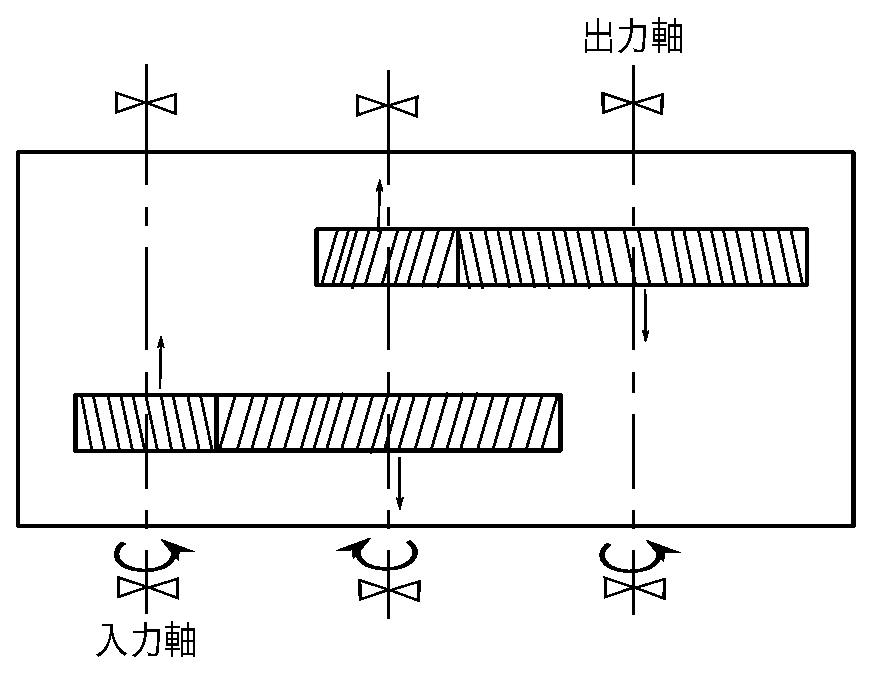
\includegraphics[width=12cm]{../picture/hagu.eps}
\end{center}
\caption{簡易平面図}
\end{figure}